\documentclass{article}
\usepackage{cmap}
\usepackage[utf8]{inputenc}
\usepackage[english,ukrainian]{babel}
\usepackage{graphicx}
\usepackage{geometry}
\usepackage{listings}
\usepackage{float}
\usepackage{multicol}
\geometry{
	a4paper,
	left=20mm,
	right=20mm,
	top=20mm,
	bottom=20mm
}
\lstset{
	language=c,
	tabsize=4,
	keepspaces,
	showstringspaces=false,
}
\graphicspath{ {./pictures} }
\setlength{\parindent}{4em}

\newcommand\subject{Алгоритми та структури даних}
\newcommand\lecturer{доцент кафедри ПЗ\\Коротєєва Т.О.}
\newcommand\teacher{асистент кафедри ПЗ\\Франко А.В.}
\newcommand\mygroup{ПЗ-22}
\newcommand\lab{8}
\newcommand\theme{ЛІНІЙНІ СТРУКТУРИ ДАНИХ }
\newcommand\purpose{познайомитися з лінійними структурами даних (стек, черга, дек, список) та отримати навички програмування алгоритмів, що їх обробляють}

\begin{document}
	\begin{normalsize}
		\begin{titlepage}
			\thispagestyle{empty}
			\begin{center}
				\textbf{МІНІСТЕРСТВО ОСВІТИ І НАУКИ УКРАЇНИ\\
					НАЦІОНАЛЬНИЙ УНІВЕРСИТЕТ "ЛЬВІВСЬКА ПОЛІТЕХНІКА"}
			\end{center}
			\begin{flushright}
				Інститут \textbf{КНІТ}\\
				Кафедра \textbf{ПЗ}
			\end{flushright}
			\vspace{200pt}
			\begin{center}
				\textbf{ЗВІТ}\\
				\vspace{10pt}
				До лабораторної роботи № \lab\\
				\textbf{На тему}: “\textit{\theme}”\\
				\textbf{З дисципліни}: “\subject”
			\end{center}
			\vspace{112pt}
			\begin{flushright}
				
				\textbf{Лектор}:\\
				\lecturer\\
				\vspace{28pt}
				\textbf{Виконав}:\\
				
				студент групи \mygroup\\
				Коваленко Д.М.\\
				\vspace{28pt}
				\textbf{Прийняв}:\\
				
				\teacher\\
				
				\vspace{28pt}
				«\rule{1cm}{0.15mm}» \rule{1.5cm}{0.15mm} 2022 р.\\
				$\sum$ = \rule{1cm}{0.15mm}……………\\
				
			\end{flushright}
			\vspace{\fill}
			\begin{center}
				\textbf{Львів — 2022}
			\end{center}
		\end{titlepage}
		
		\begin{description}
			\item[Тема.] \theme.
			\item[Мета.] \purpose.
		\end{description}
		
		\section*{Лабораторне завдання}

	Розробити програму, яка читає з клавіатури послідовність даних, жодне з яких не повторюється, зберігає їх до структури даних (згідно з варіантом) та видає на екран такі характеристики: 
		\begin{center}
			\begin{enumerate}
				\item кількість елементів;
				\item мінімальний та максимальний елемент (для символів за кодом);
				\item третій елемент з початку послідовності та другий з кінця послідовності;
				\item елемент, що стоїть перед мінімальним елементом та елемент, що стоїть після максимального;
				\item знайти позицію елемента, значення якого задається з клавіатури;
				\item об'єднати дві структури в одну.
			\end{enumerate}
		Варіант 2: стек дійсних. 
		\end{center}
		
		\section*{Теоретичні відомості}
		Стек, черга, дек, список відносяться до класу лінійних динамічних структур.
		
		Зі стеку (stack) можна видалити тільки той елемент, який був у нього доданий останнім: стек працює за принципом «останнім прийшов – першим пішов» (last-in, first-out – LIFO).
		
		З черги (queue), навпаки, можна видалити тільки той елемент, який знаходився в черзі довше за всіх: працює принцип «першим прийшов – першим пішов» (first-in, first-out – FIFO).
		
		Дек - це впорядкована лінійна динамічно змінювана послідовність елементів, у якій виконуються такі умови: 1) новий елемент може приєднуватися з обох боків послідовності; 2) вибірка елементів можлива також з обох боків послідовності. Дек називають реверсивною чергою або чергою з двома боками.
		
		У зв’язаному списку (або просто списку; linked list) елементи лінійно впорядковані, але порядок визначається не номерами, як у масиві, а вказівниками, що входять до складу елементів списку. Списки є зручним способом реалізації динамічних множин.
		
		Елемент двобічно зв’язаного списку (doubly linked list) – це запис, що містить три поля: key (ключ) і два вказівники next (наступний) і prev (попередній). Крім цього, елементи списку можуть містити додаткові дані.
		
		У кільцевому списку (circular list) поле prev голови списку вказує на хвіст списку, а поле next хвоста списку вказує на голову списку. 
		
		\section*{Хід роботи}
		\begin{lstlisting}[language=C]
	use fake::{Faker, Fake};
	
	use std::rc::Rc;
	
	#[derive(Debug)]
	pub struct Stack<T> {
		head: Link<T>,
	}
	
	type Link<T> = Option<Rc<Node<T>>>;
	
	#[derive(Debug)]
	struct Node<T> {
		elem: T,
		next: Link<T>,
	}
	
	impl<T> Stack<T> {
		pub fn new() -> Self {
			Stack { head: None }
		}
		
		pub fn push(&self, elem: T) -> Stack<T> {
			Stack { head: Some(Rc::new(Node {
					elem,
					next: self.head.clone(),
				}))}
		}
		
		pub fn pop(&self) -> Stack<T> {
			Stack { head: self.head.as_ref().and_then(|node| node.next.clone()) }
		}
		
		pub fn head(&self) -> Option<&T> {
			self.head.as_ref().map(|node| &node.elem)
		}
		
		pub fn iter(&self) -> Iter<'_, T> {
			Iter { next: self.head.as_deref() }
		}
	}
	
	impl Stack<f32> {
		pub fn new_random() -> Self {
			let stack = Stack::new();
			let stack = stack.push((f32::trunc(Faker.fake::<f32>() * 100.0)) / 100.0);
			let stack = stack.push((f32::trunc(Faker.fake::<f32>() * 100.0)) / 100.0);
			let stack = stack.push((f32::trunc(Faker.fake::<f32>() * 100.0)) / 100.0);
			let stack = stack.push((f32::trunc(Faker.fake::<f32>() * 100.0)) / 100.0);
			stack
		}
	}
	
	impl<T> Drop for Stack<T> {
		fn drop(&mut self) {
			let mut head = self.head.take();
			while let Some(node) = head {
				if let Ok(mut node) = Rc::try_unwrap(node) {
					head = node.next.take();
				} else {
					break;
				}
			}
		}
	}
	
	pub struct Iter<'a, T> {
		next: Option<&'a Node<T>>,
	}
	
	impl<'a, T> Iterator for Iter<'a, T> {
		type Item = &'a T;
		
		fn next(&mut self) -> Option<Self::Item> {
			self.next.map(|node| {
				self.next = node.next.as_deref();
				&node.elem
			})
		}
	}
			
		\end{lstlisting}
		
		\begin{figure}[H]
			\centering
			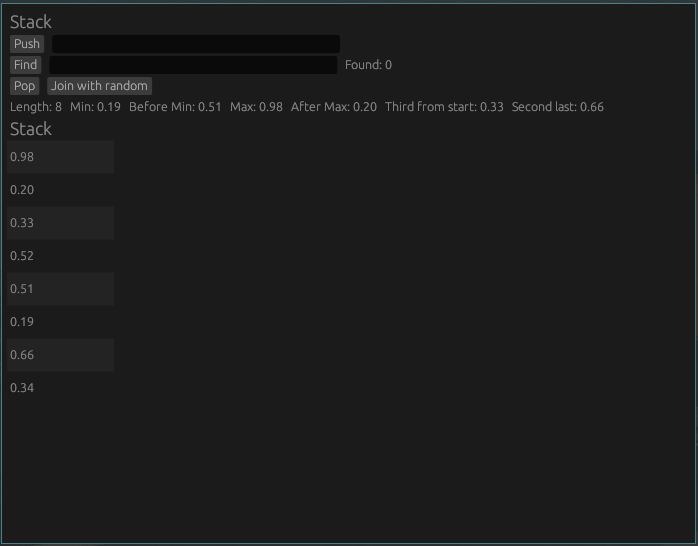
\includegraphics[scale=0.6]{1}	
			\caption{Виконання програми}
		\end{figure}
		
		\section*{Висновоки}
		Під час виконання лабораторної роботи я познайомився з лінійними структурами даних (стек, черга, дек, список) та отримав навички програмування алгоритмів, що їх обробляють
		
	\end{normalsize}
\end{document}
